\section{姿勢制御系}

\subsection{制御方式}
OrigamiSat-1 搭載の 5.8GHz 通信用パッチアンテナは指向性を持つため,同アン
テナ取付面を地上に向ける姿勢制御が必要となる.本衛星では,永久磁石と地
磁気の干渉を利用した受動的姿勢制御を採用した.飛行と姿勢のイメージを図
\ref{image_attitude_ctrl}に示す.衛星内部に搭載された棒磁石により姿勢
は地磁場の磁力線に沿う様に回転する.この過程で,日本の緯度付近を通過す
る際,パッチアンテナの面が地上を向く.但し,軌道上では運動を減衰させる
要素が乏しく,実際には磁力線を中心に揺動運動することとなる.このため,
本衛星では,PCパーマロイ製のヒステリシスダンパを搭載している.本ダンパ
は,磁力線の相対運動に伴い電磁誘導を生じ,内部抵抗による電力消費によっ
て,運動を熱に変換する.本方式は,同じく5.8GHzパッチアンテナを搭載して
いた,FITSAT-1(にわか)に採用され,実績があることから採用した.

\begin{figure}[htbp]
	\centering
	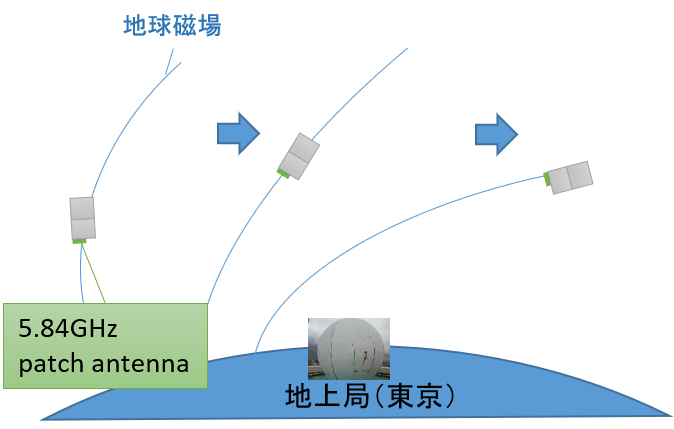
\includegraphics[width=10cm]{./03/fig/image_attitude_ctrl.png}
	\caption{飛行と姿勢のイメージ}
	\label{image_attitude_ctrl}
\end{figure}

\subsection{主要諸元}
本衛星の姿勢制御用永久磁石およびヒステリシスダンパの搭載イメージを図
\ref{image_mag_HD}に示す.また,それぞれの諸元を表
\ref{spec_magnet}, 表\ref{spec_HD}に示す.

\begin{figure}[htbp]
	\centering
	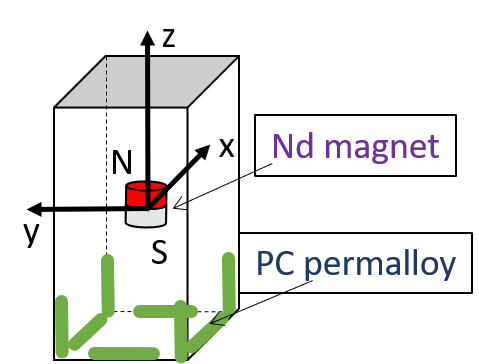
\includegraphics[width=5cm]{./03/fig/image_mag_HD.png}
	\caption{永久磁石とヒステリシスダンパ搭載イメージ}
	\label{image_mag_HD}
\end{figure}

\begin{table}[htb]
    \centering
    \caption{OrigamiSat-1搭載磁石諸元}
    \label{spec_magnet}
    \begin{tabular}{cc} \hline
      項目 & 諸元 \\ \hline\hline
      材質 & Nd \\
        体積 & $2.73 \times 10^{-6} [\rm{m^3}]$\\ 
        磁束密度 & 0.468 [T] \\ 
        発生トルクオーダー & $10^{-5}$ [Nm] \\ \hline   
    \end{tabular}
    \label{requirment_op}
\end{table}

\begin{table}[htb]
    \centering
    \caption{OrigamiSat-1 搭載ヒステリシスダンパ諸元}
    \label{spec_HD}
    \begin{tabular}{cc} \hline
      項目 & 諸元 \\ \hline\hline
        材質 & PC パーマロイ \\
        体積(X-axis) & 1.603 $\times 10^{-7} [\rm{m^3}]$ \\
        体積(Y-axis) & 1.320 $\times 10^{-7} [\rm{m^3}]$ \\
        体積(Z-axis) & 5.055 $\times 10^{-8} [\rm{m^3}]$ \\
        飽和磁束密度 & 0.65 [T] \\
        残留磁束密度 & 0.40 [T] \\
        保磁力 & 1.2 [A/m] \\
        発生トルクオーダー & $10^{-6}$ [Nm] \\ \hline    
    \end{tabular}
    \label{requirment_op}
\end{table}

\subsection{姿勢解析}
衛星の回転運動に関する運動方程式は,次式で表される.
\begin{equation}
  \bm{I} \dot{\bm{\omega}} + \bm{\omega} \times \bm{I} \bm{\omega} = \bm{T}
\end{equation}

ここで,$\bm{I}$は慣性テンソル,$\bm{\omega}$は角速度,$\bm{T}$は外力
トルクである.本衛星では,地磁気と永久磁石による磁気トルク $\bm{T}_{m}$,
地磁気とヒステリシスダンパによる磁気トルク $\bm{T}_{d}$,空気抵抗によるトルク
$\bm{T}_{air}$,太陽光輻射圧トルク $\bm{T}_{sun}$,重力傾斜トルク
$\bm{T}_{g}$ を想定し,$\bm{T}$ を式\ref{3_5_torque}で与える.
\begin{equation}
  \bm{T} = \bm{T}_{m} + \bm{T}_h + \bm{T}_{sun} + \bm{T}_{air} + \bm{T}_{g} \label{3_5_torque}
\end{equation}

\subsubsection{磁気トルク}
地磁気と衛星搭載磁石により発生するトルクは,磁石の磁気モーメント
$\bm{M}_m$ と 地球磁場 $\bm{H}$ により次式で表される.
\begin{eqnarray}
  \bm{T}_{m} = \bm{M}_{m} \times \bm{H} \\
  \bm{M}_m = \frac{V_m}{\mu_0} \bm{B_m}
\end{eqnarray}
ここで,$V_m$は磁石の体積, $\mu_0$は真空の透磁率,$\bm{B_m}$は磁石の
磁束密度ベクトルである.

\subsubsection{ヒステリシスダンパ}
常磁性体は外部磁場により磁化された後,図\ref{3_5_hysteresis_loop}に示
すように,外部磁場が減少し0になっても,磁化(磁束密度)が残留する(ヒス
  テリシスを持つ).このヒステリシスループを巡る過程でエネルギー損失が
発生し,ダンパとして作用する.

\begin{figure}[htbp]
	\centering
	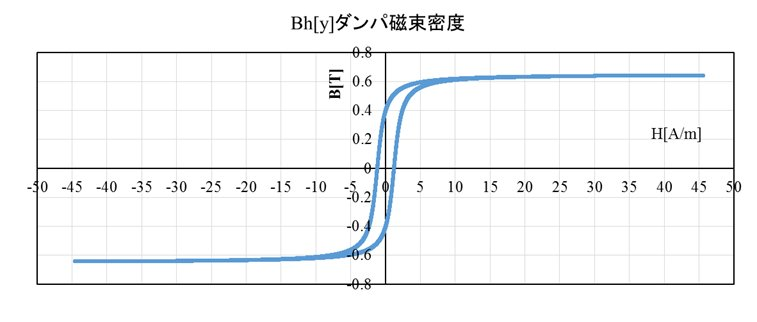
\includegraphics[width=8cm]{./03/fig/3_5_hysteresis_loop.jpg}
	\caption{磁性体のヒステリシス}
	\label{3_5_hysteresis_loop}
\end{figure}

ヒステリシスダンパの磁束密度$B_h$は,地球磁場により次式のように与えられる.
\begin{equation}
B_h = \frac{2B_s}{\pi}\tan^{-1}\left[\frac{1}{H_0}\tan\left(\frac{\pi
    B_0}{2B_s}\right)(H \pm H_0) \right]
\end{equation}
ここで,$B_s$, $B_0$, $H_0$ はそれぞれヒステリシスダンパの飽和磁束密度,
残留磁束密度,保持力である.
この時,ヒステリシスダンパトルク$\bm{T}_h$は,
\begin{eqnarray}
  \bm{T}_{h} = \bm{M}_{h} \times \bm{H} \\
  \bm{M}_h = \frac{V_h}{\mu_0} \bm{B_h}
\end{eqnarray}
となる.ここで $\bm{M}_h$,$V_h$は,それぞれヒステリシスダンパの磁気モー
メント,体積である.
永久磁石とヒステリシスダンパのサイジングについては,後述のシミュレーション結果に基づく
遺伝的アルゴリズムにより決定した.

\subsubsection{太陽光輻射トルク}
光圧は,鏡面反射,拡散反射,吸収によって異なり,それぞれの単位面積当た
りの光圧 $d \bm{f}_a$, $d \bm{f}_s$, $d \bm{f}_d$, はそれぞれ次式で表
される.
\begin{eqnarray}
  d \bm{f}_a &=& -M_s\rho_a(\bm{s} \cdot \bm{n})\bm{s}dA  \\
  d \bm{f}_s &=& -2M_s\rho_s (\bm{s} \cdot \bm{n})^2
  \bm{n}dA \\
  d \bm{f}_d &=& -M_s\rho_d (\bm{s} \cdot \bm{n}) \left(\bm{s} +
  \frac{2}{3}\bm{n} \right) dA
\end{eqnarray}
ここで,$\rho_a$, $\rho_s$, $\rho_d$ はそれぞれ,光の吸収率,鏡面反射
率,拡散反射率であり,光が透過しない材料では以下の関係を持つ.
\begin{equation}
  \rho_a + \rho_s + \rho_d = 1
\end{equation}
また,$\bm{s}$は太陽方向ベクトル, $\bm{n}$は衛星表面の法線ベクトル,
$A$は照射面積である.
$M_s$ は,次式で定義される.
\begin{equation}
  M_s = \frac{E_s}{c} \cdot \left( \frac{AU}{r_{sun}} \right)^2
\end{equation}
ここで,$E_s$, $c$, $AU$, $r_{sun}$はそれぞれ,太陽定数,光速,地球-太
陽間距離,衛星-太陽間距離である.
これらを用いて,太陽光輻射圧トルクは次式で与えられる.
\begin{equation}
  \bm{T}_{sun} = \int_{\bm{s}\cdot\bm{n}} \bm{r} \times \nu(d\bm{f}_a +
  d\bm{f}_s + d\bm{f}_d)
\end{equation}
ここで $\nu$ は日照条件である.(日照: $\nu=1$, 日陰: $\nu=0$).


\subsubsection{空気抵抗トルク}
空気抵抗トルクは次式で与えられる
\begin{equation}
  \bm{T}_{air} = \int_{\bm{n}\cdot\bm{v}} \bm{r} \times
  -\frac{1}{2}C_d\rho (\bm{n}\cdot\bm{v})\bm{v} dA
\end{equation}
ここで,$\bm{r}$は衛星重心から空力中心への位置ベクトル,$C_d$ は空気抵
抗係数,$\rho$ は大気密度,$\bm{v}$ は衛星の速度ベクトルである.

\subsubsection{重力傾斜トルク}
重力傾斜トルクは,次式で与えられる.
\begin{equation}
  \bm{T}_g = -\frac{3\mu}{|\bm{r_e}|^3}\bm{r_e} \times (\bm{I} \cdot
  \bm{r_e})
\end{equation}
ここで,$\mu$は地球重力定位数,$\bm{r_e}|$は地球重心から衛星重心への位
置ベクトル,$\bm{I}$は衛星の慣性テンソルである.

\subsection{解析結果}
上記の式に基づき,地球周回時の OrigamiSat-1 の姿勢についてシミュレーショ
ンを行った.地球磁場については,国際地球電磁気学会の標準磁場モデルであ
る IGRF (International Geomagnetic Reference Field) を用いた.
また,大気モデルとして Harris Priester Model を用いた.

以下,各条件におけるOrigamiSat-1の運動予測について結果を示す.
各軸方向は,図\ref{image_mag_HD}の通りである.

\subsubsection{3U 膜展開前}
E-SSODより放出された直後を想定し,3U状態,膜面未展開,マスト伸展無し,
高度500km,初期角速度が全軸 0 という条件における角速度および,
機体z軸と地球磁力線とのなす角をそれぞれ図\ref{3_5_sim_3udep_angvel}と
図\ref{3_5_sim_3udep_zang}に示す.放出からおよそ16000秒程度で姿勢が安
定している.

\begin{figure}[htbp]
	\centering
	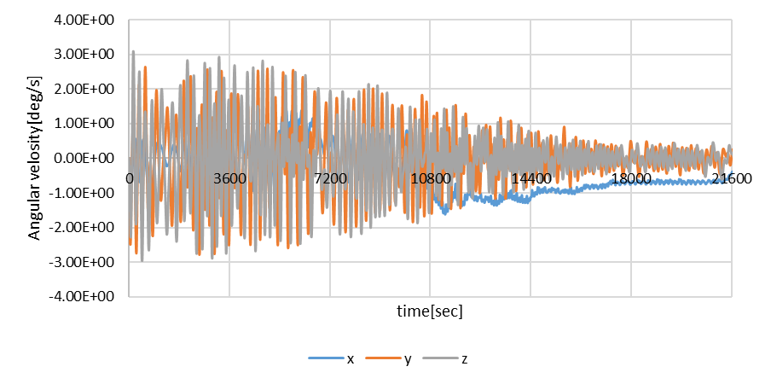
\includegraphics[width=9cm]{./03/fig/3_5_sim_3udep_angvel.png}
	\caption{放出直後の角速度推移(初期角速度無し)}
	\label{3_5_sim_3udep_angvel}
%\end{figure}
%\begin{figure}[htbp]
	\centering
	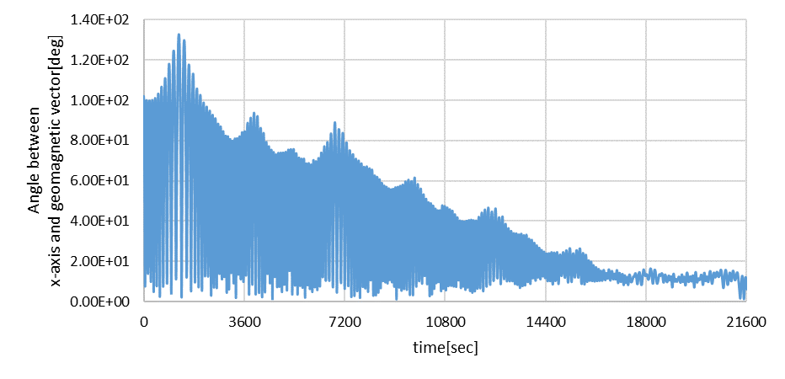
\includegraphics[width=9cm]{./03/fig/3_5_sim_3udep_zang.png}
	\caption{放出直後の機体z軸と地球磁場のなす角度の推移 (初期角速
          度無し)}
	\label{3_5_sim_3udep_angvel}
\end{figure}

また,初期角速度を,x軸: 30deg/s, y軸: 30deg/s, z軸: 5deg/s,とした場
合についての結果を図\ref{3_5_sim_3udep_angvel2}と
図\ref{3_5_sim_3udep_zang2}に示す.この条件においても,静定に数日を要
するものの,姿勢は静定する.

\begin{figure}[htbp]
	\centering
	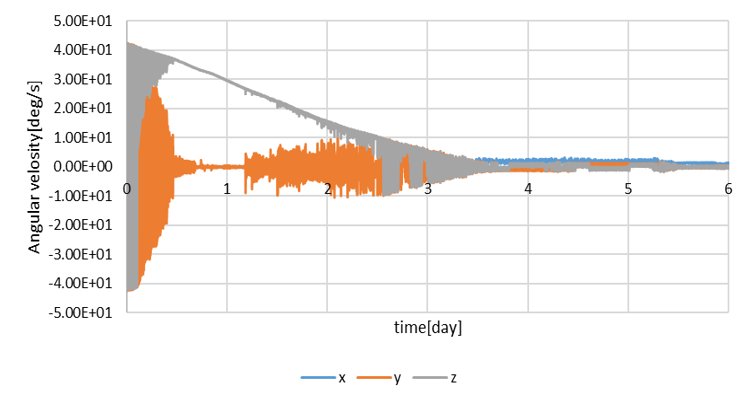
\includegraphics[width=9cm]{./03/fig/3_5_sim_3udep_angvel2.png}
	\caption{放出直後の角速度推移 (初期角速度あり)}
	\label{3_5_sim_3udep_angvel2}
%\end{figure}
%\begin{figure}[htbp]
	\centering
	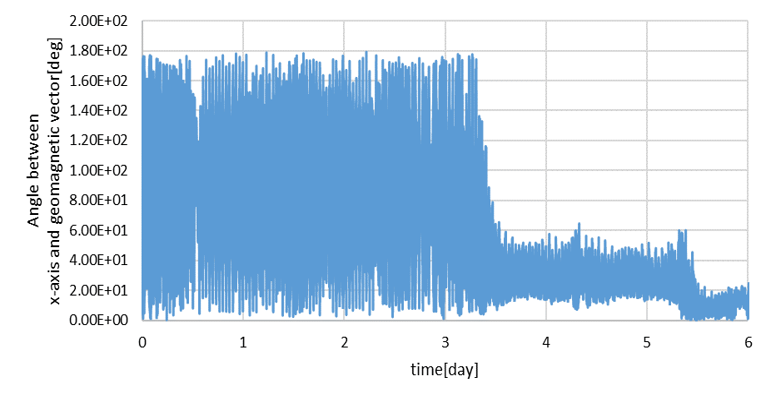
\includegraphics[width=9cm]{./03/fig/3_5_sim_3udep_zang2.png}
	\caption{放出直後の機体z軸と地球磁場のなす角度の推移 (初期角速
          度あり)}
	\label{3_5_sim_3udep_angvel2}
\end{figure}

\subsubsection{2U 膜切り離し後}
ミッションの後半.マストおよび膜切り離し後に2U状態となった際の運動につ
いて,機体の慣性条件が変化しても姿勢安定が成立するかを検討した.2U状態,高度400km,初期角速度が全軸 0 という条件における角速度および,
機体z軸と地球磁力線とのなす角をそれぞれ図\ref{3_5_sim_2u_angvel}と
図\ref{3_5_sim_2u_zang}に示す.2Uの状態においても,放出からおよそ10000秒程度で姿勢が安
定している.

\begin{figure}[htbp]
	\centering
	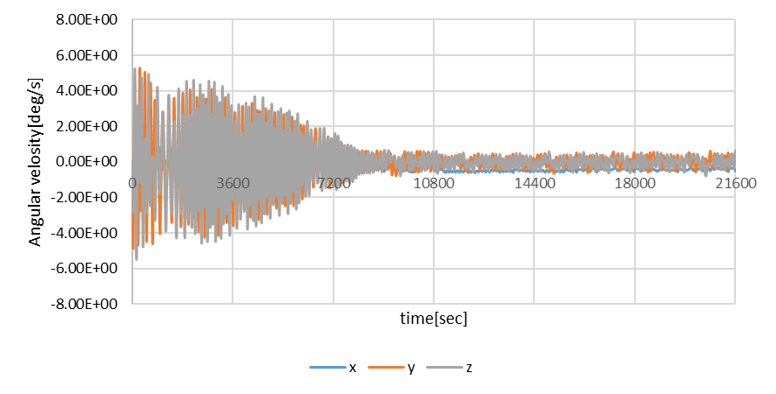
\includegraphics[width=9cm]{./03/fig/3_5_sim_2u_angvel.png}
	\caption{膜切り離し後の角速度推移}
	\label{3_5_sim_2u_angvel}
%\end{figure}
%\begin{figure}[htbp]
	\centering
	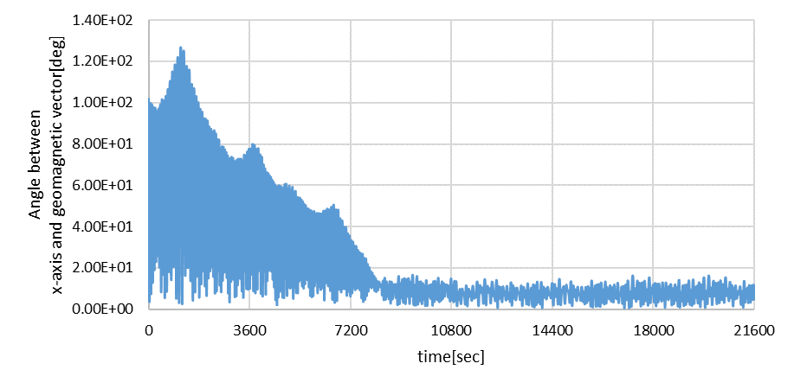
\includegraphics[width=9cm]{./03/fig/3_5_sim_2u_zang.png}
	\caption{膜切り離し後の機体z軸と地球磁場のなす角度の推移}
	\label{3_5_sim_2u_zang}
\end{figure}

\subsubsection{3U 膜展開時}
膜展開状態は,空力,太陽光輻射,重力傾斜各トルクの外乱が大きくなること
が予想されるが,この状態おいても姿勢安定が可能であれば,5.8GHz高速通信
が可能となる.3U状態,高度500km,マスト伸展状態,初期角速度が全軸 0 という条件における角速度および,機体z軸と地球磁力線とのなす角をそれぞれ図\ref{3_5_sim_membrane_angvel}と
図\ref{3_5_sim_membrane_zang}に示す.こちらは角速度が発散することは無
く,$10^{-1}$deg/sオーダーの運動となっているが,姿勢は安定せず5.8GHzパッ
チアンテナを地上に向け続けることは困難であることが判明した.本結果に基
づき,5.8GHz高速通信については膜切り離し後に実施することとし,それまで
大容量の実験データは機体上に保存しておくこととした.

\begin{figure}[htbp]
	\centering
	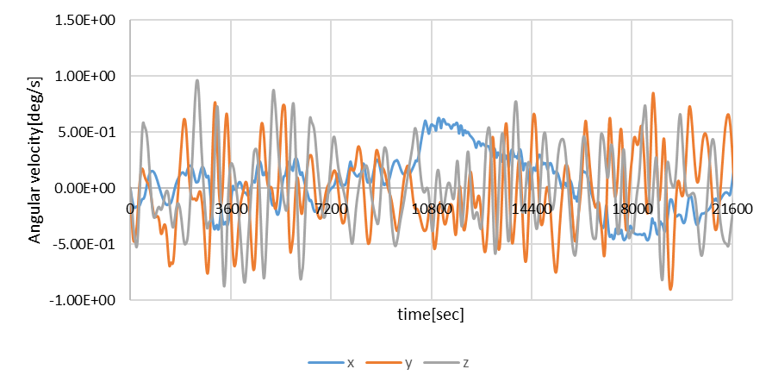
\includegraphics[width=9cm]{./03/fig/3_5_sim_membrane_angvel.png}
	\caption{膜展開時の角速度推移}
	\label{3_5_sim_membrane_angvel}
%\end{figure}
%\begin{figure}[htbp]
	\centering
	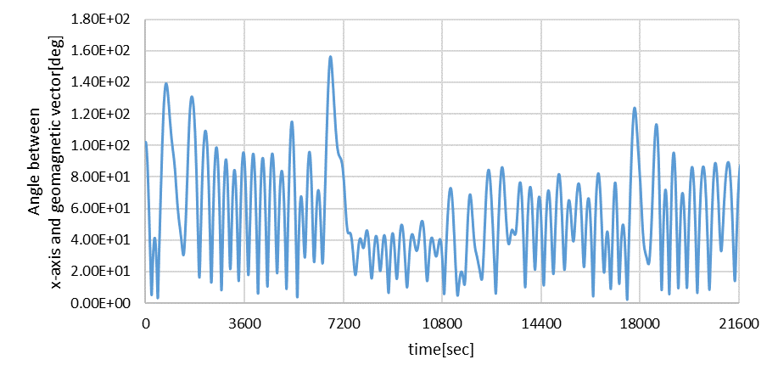
\includegraphics[width=9cm]{./03/fig/3_5_sim_membrane_zang.png}
	\caption{膜展開時の機体z軸と地球磁場のなす角度の推移}
	\label{3_5_sim_membrane_zang}
\end{figure}
